\documentclass[]{article}

\usepackage{amssymb} \usepackage{graphicx} \graphicspath{ {../imgs/} }

\title{Graph Search-Based Path Planning with moving Obstacles using Persistent Homology}
\author{Daniel Bencic}
\date{28.10.2022}

\begin{document}
\maketitle

\section{Introduction} One of the crucial tasks for every autonomous
robot is finding a collision free path through free space. Due to it's
importance this problem has been studied for decades and is know as
the path planning or the ``piano movers'' problem
\cite{schwartzPianoMoversProblem1983a,schwartzPianoMoversProblem1983b}.
While there exist polynomial time algorithms for very simple planning
problems, the general path planning problem is PSPACE-complete
\cite{reifComplexityMoverProblem1979}. The problem becomes
computationally even harder if obstacles are not static anymore and
the additional dimension of time is added to the
problem. It has already been shown that the understanding of the
topological strucuture of the configuration space can be used to
improve algorithm performance by reducing the search space and solving
the path planning problem on a more abstract level.

\section{Problem Formulation}
\subsection*{Preliminaries} This section introduces some fundamental
concepts of topology and path planning
\cite{munkresTopology2014,lavallePlanningAlgorithms2006,hatcherAlgebraicTopology2002,
otterRoadmapComputationPersistent2017}.

\textbf{Homeomorphism} If there exists a bijective function
\(f: X \mapsto Y\) such that \(f\) and it's inverse \(f^{-1}\) are
continuous functions, then the topological spaces \(X\) and \(Y\) are
homeomorphic. Homeomorphism implies that both \(X\) and \(Y\) share
the same topological properties.

\textbf{Configuration Space} Given a metric space \(\mathcal{W}\) with
metric \(d\) and a rigid body \(\mathcal{A}\), a rigid body
transformation is a function \(f: \mathcal{A} \mapsto \mathcal{W}\)
such that \(d(a_{1}, a_{2}) = d(f(a_{1}), f(a_{2}))\) and no
reflection occurs. This holds for rotations and translations. Given
\(GL(n)\) by the set of all invertible \(n \times n\) matrices,
\(O(n)\) is a subgroup of \(GL(n)\) such that \(QQ^{T} = Q^{T}Q = I\)
for all \(Q \in O(n)\). The subgroup \(SO(n)\) of \(O(n)\) which
contains all rotations matrices meaning \(det(P) = 1\) for all
\(P \in SE(n)\). Combining arbitrary rotations and translations gives
the special euclidean group \(SE(n)\) which is homeomorphic to
\(\mathbb{R}^{n} \times SO(n)\).

The configuration space for a rigid robot is therefore
\(\mathcal{C} \cong \mathbb{R}^{2} \times \mathbb{S}^{1}\) and
\(\mathcal{C} \cong \mathbb{R}^{3} \times \mathbb{RP}^{3}\) in 2D
space and 3D space, respectively.

\textbf{Path} Given two points \(x_{0}, x_{1} \in X\), a path is a
continous function \(f: [0, 1] \mapsto X\) such that \(f(0) = x_{0}\)
and \(f(1) = x_{1}\). Paths for which \(f(0) = f(1) = x_{0}\) are
loops with basepoint \(x_{0}\).

\textbf{Homotopy} Two paths \(f\) and \(g\) with the same initial and endpoints
are homotopic if one can be continuously deformed into the
other. Formally, there exists a familiy
\(f_{t}: [0, 1] \mapsto X, 0 \le t \le 1\) such that
\(f_{t}(0) = x_{0}\), \(f_{t}(1) = x_{1}\) and \(f_{0}(s) = f(s)\),
\(f_{1}(s) = g(s)\) and the function
\(F(s, t): [0, 1] \times [0, 1] \mapsto X\) defined by
\(F(s, t) = f_{t}(s)\) is continuous (Figure \ref{fig:homotopy}).

\begin{figure}[h] \centering 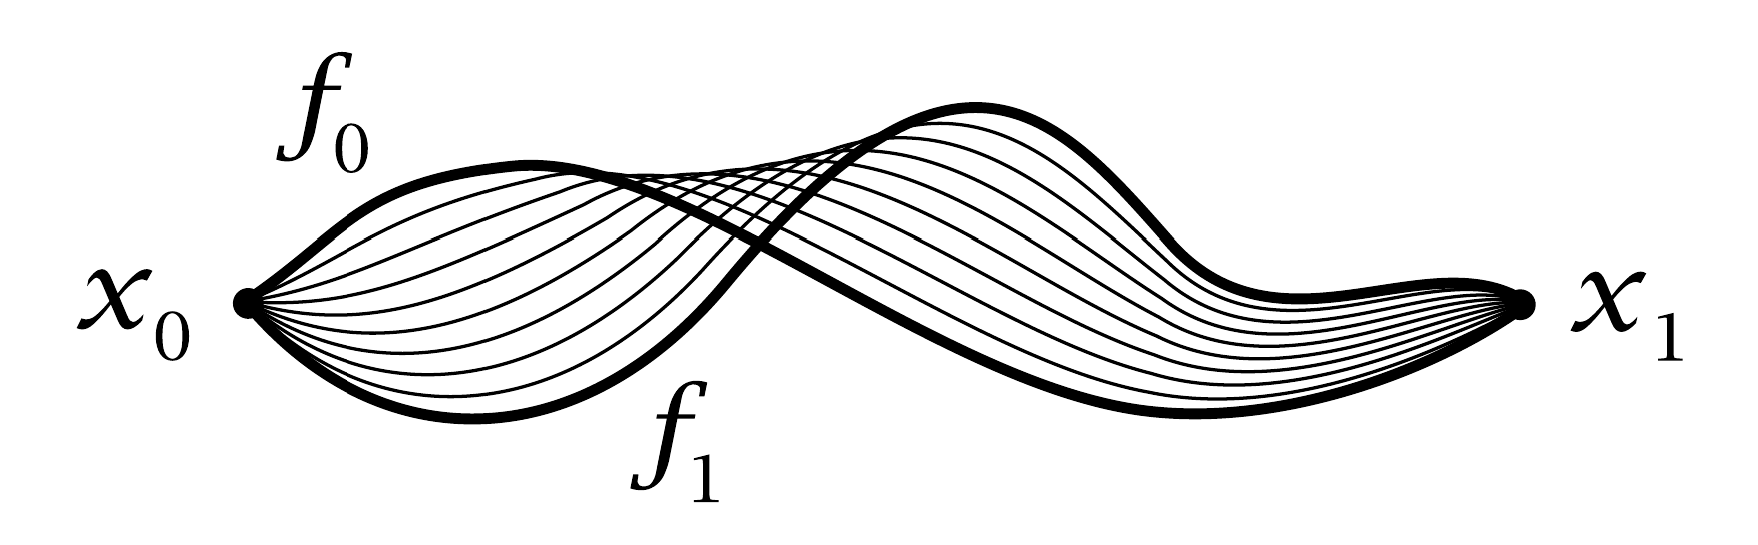
\includegraphics[scale=.18]{homotopy}
  \caption{Homotopy \cite{hatcherAlgebraicTopology2002}.}
  \label{fig:homotopy}
\end{figure}

\textbf{Simplicial Complex} A simplicial complex is a collection \(K\) of
subsets of a set \(K_{0}\) such that \(\{v\}\ \in K\) for all \(v \in
K_{0}\) and if \(\tau \subset \sigma\) and \(\sigma \in K\), \(\tau
\in K\). The elements of \(K_{0}\) are called vertices and the
elements of \(K\) are called simplices. A simplex \(\sigma \in K\) is
called p-simplex if \(|\sigma| = p + 1\). The collection of all
p-simplices is denoted as \(K_{p}\). The k-skeleton of \(K\) is the
union of all \(K_{p}\) for \(p = \{1, 2, ..., k\}\). A simplex \(\tau\)
is called a face of simplex \(\sigma\) if \(\tau \subset
\sigma\). Figure \ref{fig:simplicialcomplex} shows and example for \(K = \{\{a\}, \{b\}, \{c\}, \{d\}, \{a,
    b\}, \{a, c\}, \{a, d\}, \{b, c\}, \{c, d\}, \{a, b, c\}\}\).

\begin{figure}[h] \centering 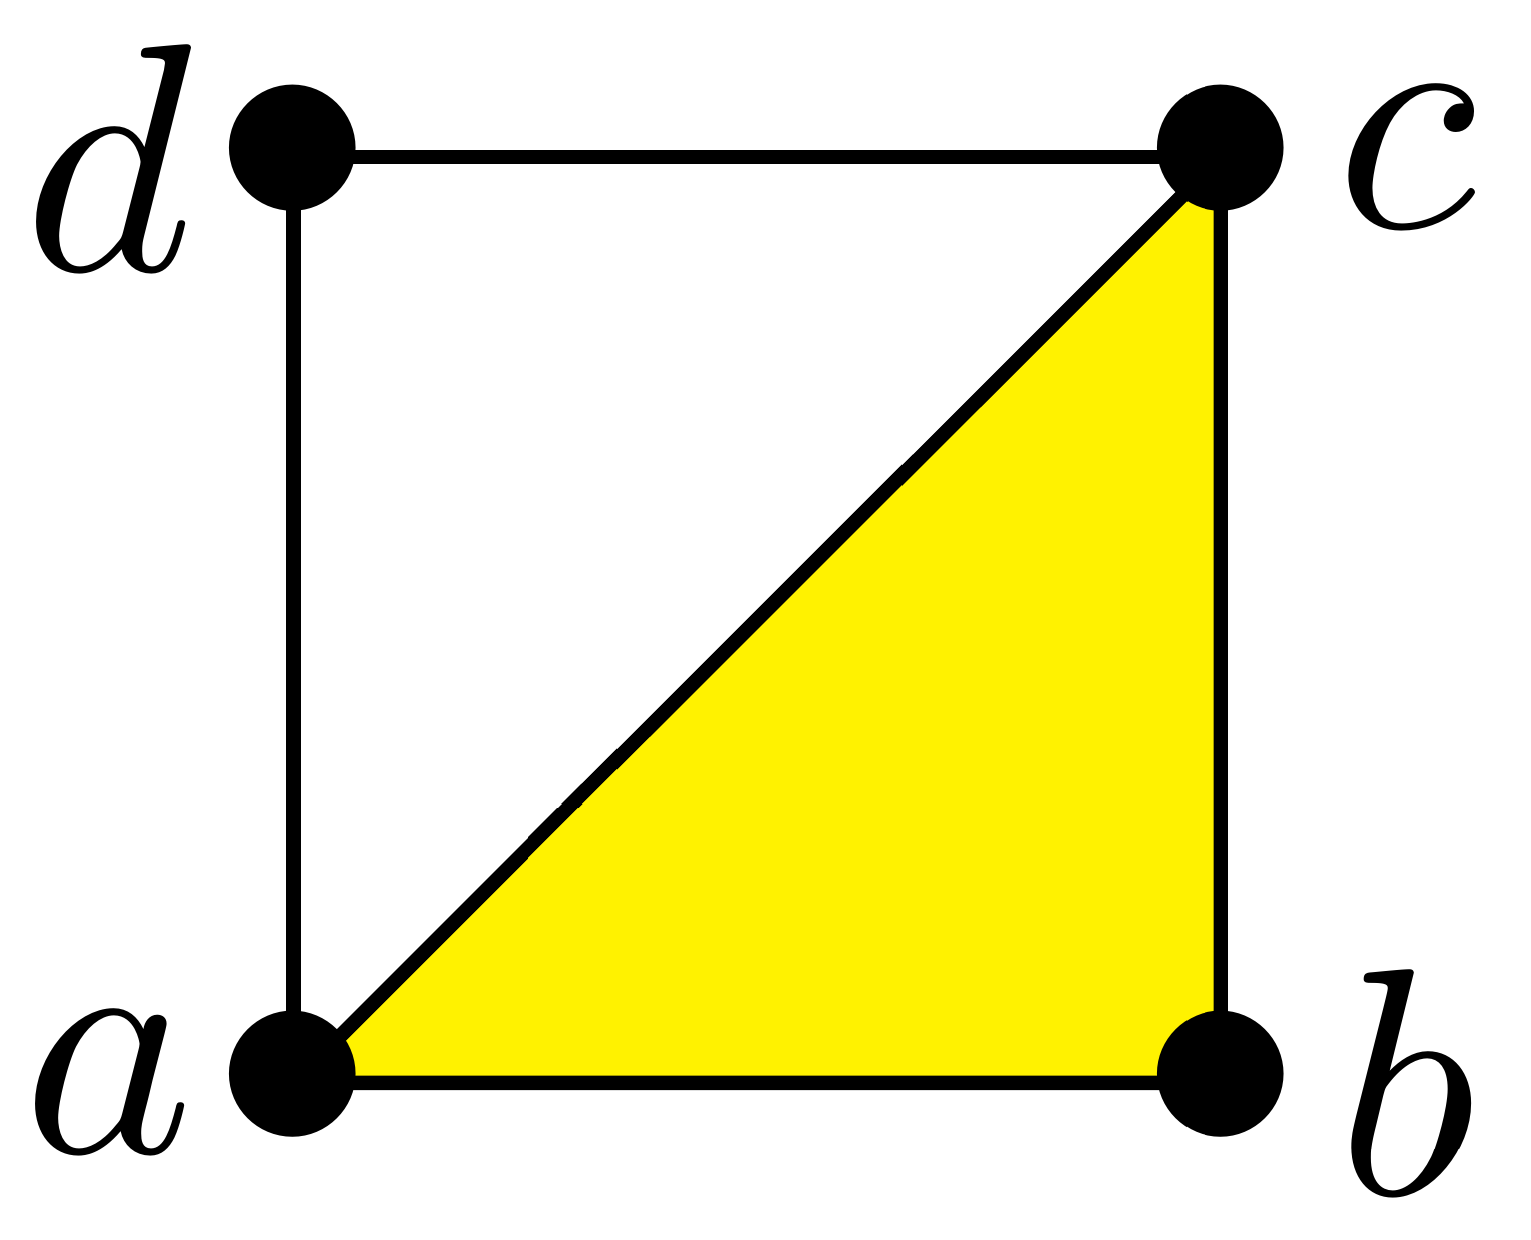
\includegraphics[scale=.10]{simplicialcomplex}
  \caption{Simplicial complex \cite{otterRoadmapComputationPersistent2017}.}
  \label{fig:simplicialcomplex}
\end{figure}

\textbf{Persitent Homology}

\subsection*{The Path Planning Problem} We use the definition of a
path planning problem introduced by Farber
\cite{farberTopologicalComplexityMotion2003}. Given a map \(\pi: PX
\mapsto X \times X\) that associates with every path \(\gamma \in PX\)
the pair of it's initial and endpoints \(\pi(\gamma) = (\gamma(0),
\gamma(1))\), path planning is finding a function \(s: X \times X
\mapsto PX\) such that the composition \(\pi \circ s = id\). A
continuous path planning is then given if close intial-end pairs
produce close movements (see Figure \ref{fig:continuouspathplanning}).

\begin{figure}[h]
  \centering
  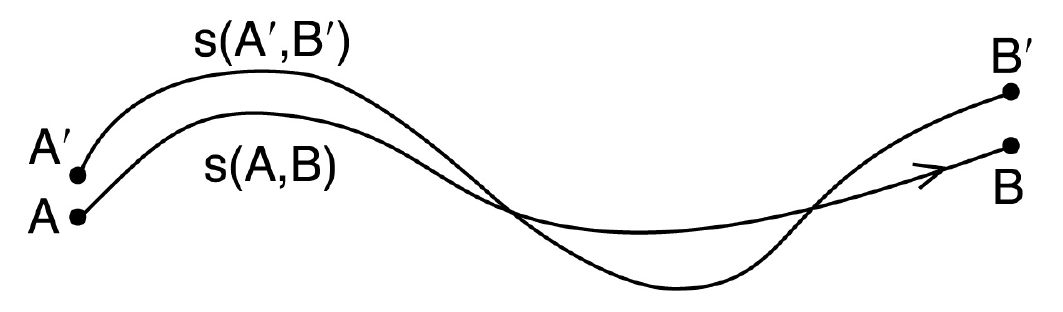
\includegraphics[scale=.3]{continuouspathplanning}
  \caption{Continuous path planning \cite{farberTopologicalComplexityMotion2003}.}
  \label{fig:continuouspathplanning}
\end{figure}

An algorithm that solves the path planning problem is said to be
\textit{complete} if it finds a solution if there exists one and
returns failure otherwise. It is called \textit{optimal} if the
returned path minimizes a cost metric. For sampling-based algorithms
the theoretical guarantees are weakened. An algorithm is called
\textit{probabilistic complete} if the probability that it fails to
return a solution if one exists decays to zero as the number of
samples approaches infinity. It is called \textit{asymptotically
  optimal} if the solution converges to the optimal solution as the
number of samples approaches infinity.

\section*{Related Work}
\subsection*{Static Obstacles}
\textbf{Graph search}. These approaches assume that \(\mathcal{C}\) is
in the form of a graph. They then apply graph search techniques to
find the path \(\pi\). A widely used algorithm to compute shortest
paths in a graph is Dijkstra's algorithm
\cite{dijkstraNoteTwoProblems1959}. It is a greedy algorithm that
computes the shortest path from every node to every other node in the
graph. The next node for expansion is selected based on the lowest
cost-to-come \(\hat g(x)\). It is \textit{complete}, meaning it finds
a solution if one exists and reports failure otherwise. It is also
\textit{optimal} in the sense that the computed path is the shortest
possible path.

A* \cite{hartFormalBasisHeuristic1968} improves Dijkstra's algorithm
by reducing the number of expanded nodes in the graph. This is
achieved by using a different function
\(\hat f(x) = \hat g(x) + \hat h(x)\) to select the next node for
expansion. The term \(\hat h(x)\) is a heuristic for the least
possible cost-to-go in a metric space. Many path planning algorithms
in the current literature build upon A* (Figure
\ref{fig:graph-search}).

\begin{figure}[h] \centering
  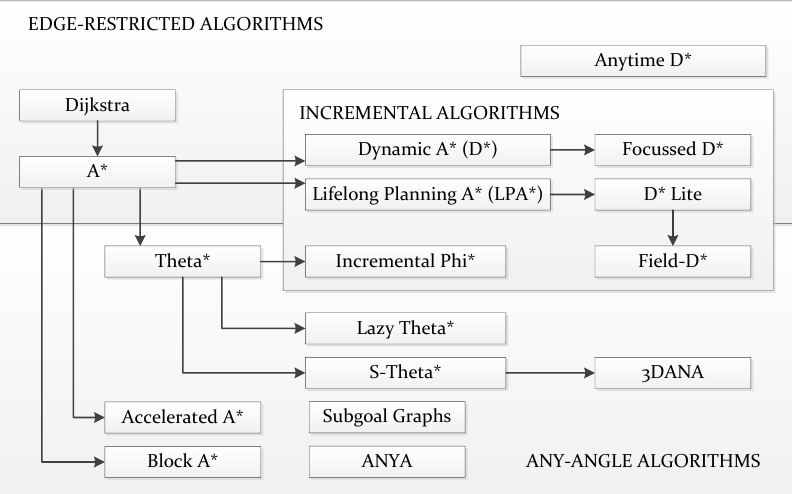
\includegraphics[scale=.35]{graph_search_algorithms}
  \caption{Evolution of graph search algorithms for the path planning
    problem \cite{sanchez-ibanezPathPlanningAutonomous2021}.}
  \label{fig:graph-search}
\end{figure}

Stentz et al. developed D*, an incremental algorithm based on A* that
is able to find shortest paths on maps with changing costs, i.e. due
to a robot moving trough the environment and updating the map. D*
computes a path backwards from the goal to the robot. Koenig et
al. \cite{koenigIncremental2001} also proposed an incremental version
of A* (LPA*), where successive runs only recalculate locally
inconsistent nodes. They combined it with the backward search of D*
and created D*-Lite \cite{koenigLite2002}, a less complex version of
D* with at least the same performance therefore making D* obsolete.

Daniel et al. \cite{danielThetaAnyAnglePath2010} showed an approach
specifically for grid-maps that is not limited to predefined angles
for the transition to other grid cells. It is based on A* and uses
line of sight to determine successor nodes. Another any-angle approach
proposed by Ferguson et al.  \cite{fergusonFieldAlgorithmImproved2005}
uses linear interpolation to find the least cost path trough a cell
and produces globally smooth paths.

A comprehensive review of graph search algorithms for the path
planning problem can be found in the literature
\cite{aitsaadiUAVPathPlanning2022,sanchez-ibanezPathPlanningAutonomous2021,yanComprehensiveSurveyAnalysis2020,nashAnyAnglePathPlanning2013}.

\textbf{Sampling}. Due to the curse of dimensionality
\cite{bellmanDynamicProgramming1984}, graph search in high dimensional
configuration spaces can quickly become computationally intractable.
Sampling-based approaches discretize the high-dimensional
configuration space by generating random samples in
\(\mathcal{C}_{free}\). One highly influential contribution from
Kavraki et. al. \cite{kavrakiProbabilisticRoadmapsPath1996} is called
Probabilistic Roadmap Method (PRM). It is a solution to the
multi-query path planning problem in high dimensional configuration
spaces. The method consists of a learning and a query phase. The
former repeatedly generates a random configuration in
\(\mathcal{C}_{free}\) and connects this sample to neighboring nodes
in a given radius with a fast local planner. In addition, a heuristic
is used to generate extra nodes in ``difficult'' regions of
\(\mathcal{C}_{free}\). The method is therefore influenced by the
topological properties of \(\mathcal{C}_{free}\). The result is a
graph representation of \(\mathcal{C}_{free}\) in the form of a forest
of trees.

Another highly cited approach using only a single tree is the
Rapidly-exploring Random Tree (RRT) algorithm by Lavalle
\cite{lavalleRapidlyExploringRandomTrees1998}. The algorithm grows a
tree in \(\mathcal{C}_{free}\) by generating a sample from a uniform
distribution and growing the nearest node of the tree in the direction
of the sample. Since the probability that a node is selected for
expansion is proportional to the size of it's Voronoi cell (see Figure
\ref{fig:rrt}), the tree grows with a bias towards unexplored regions
in \(\mathcal{C}_{free}\).

\begin{figure}[h] \centering 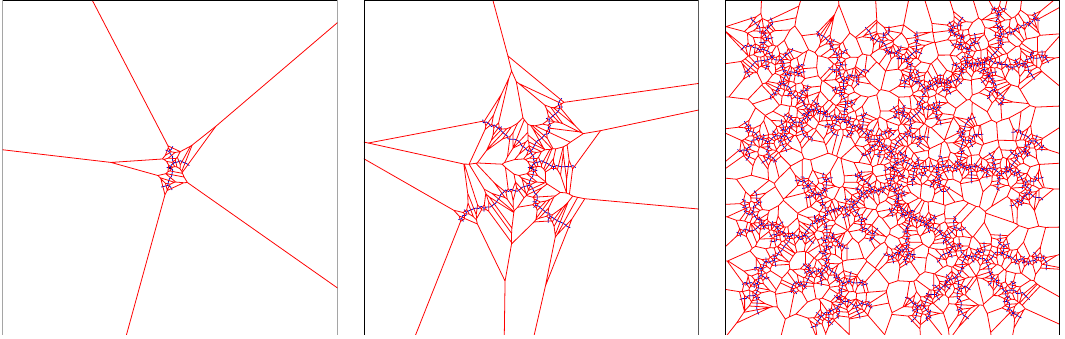
\includegraphics[scale=.275]{rrt_voronoi}
  \caption{Voronoi diagram of a RRT tree.}
  \label{fig:rrt}
\end{figure}

Karaman et. al. \cite{karamanSamplingbasedAlgorithmsOptimal2011}
showed that both PRM and RRT algorithms are not asymptotically
optimal. That means that with a growing number of nodes the
probability that the algorithm finds an optimal solution converges to
zero. In their paper they also proposed two new algorithms PRM* and
RRT* which are shown to be asymptotically optimal. The former was
improved by calculating the radius, in which a sample is connected to
it's neighbors, based on the number of present samples. The latter was
improved by selecting the node for expansion based on the cost-to-come
in the neighborhood of a sample and rewiring the tree after insertion
of a new node.

There are many algorithms improving and extending RRT and RRT* in the
literature. With RRT-Connect, Kuffner et. al.
\cite{kuffnerRRTConnectEfficientApproach} introduced a bidirectional
RRT that grows one tree from \(q_I\) and another tree from \(q_G\)
while trying to connect the two trees. Anytime RRT*
\cite{karamanAnytimeMotionPlanning2011} returns a fast initial
solution and a robot commits to execute a subset of the full path
\(\pi_{com}: [0, t_{com}] \mapsto C_{free}\). While executing
\(\pi_{com}\) the remaining path is further improved until the robot
commits to the next subset of the path. Realizing that there is a
subset of \(C_{free}\) that contains configurations that are
guaranteed to improve the current solution, Informed RRT*
\cite{gammellInformedRRTOptimal2014} uses a ellipsoidal heuristic to
sample from this set and improve the convergence rate of RRT*. BIT*
\cite{gammellBatchInformedTrees2015} does not sample a single
configuration, instead it samples a batch of configurations and grows
a tree from this batch.  After finding a solution or no further
possible expansion, the next batch is sampled. If a solution has been
found with the previous batch, this batch is sampled from the
ellipsoidal subset introduced by Informed RRT* and the tree is updated
by identifying locally inconsistent nodes.

A comprehensive review of RRT* variants has been published by Noreen
et. al.  \cite{noreenOptimalPathPlanning2016a} and a review of more
sampling-based approaches for the path planning problem can be found
in \cite{elbanhawiSamplingBasedRobotMotion2014}.

\subsection*{Homotopy Invariants}
Since the homotopy of paths forms
an equivalence relation \cite{hatcherAlgebraicTopology2002} it
partitions the set of paths for a given initial-endpoint
pair.

Bhattachary
et. al. \cite{bhattacharyaSearchbasedPathPlanning2010,bhattacharyaSearchBasedPathPlanning2012}
construct an augmented graph that can then be searched with classic
graph search algorithms. Given a graph \(G = (V, E)\), the augmented
graph is a lift of \(G\) into the covering space of \(X\). In
configuration spaces homeomorphic to \(\mathbb{R}^{2}\) they use
Cauchy's Integral Theorem and the Residue Theorem from complex
analysis to calculate a \(L\)-value which is equal for paths in the
same homtopy classes and not equal otherwise. In configuration spaces
homeomorphic to \(\mathbb{R}^{3}\) they use laws from electromagnetism
to calculate a \(H\)-value. These values are then used to augment the
respective graphs.  They propose another method to augment a graph in
\cite{bhattacharyaPathHomotopyInvariants2018}.  Here homotopy
invariants for a \(D\)-dimensional manifold \(X\) are constructed by
introducing \((D - 1)\)-submanifolds. Words are then formed by tracing
a path \(f\) and inserting a letter every time \(f\) intersects one of
the submanifolds.

\begin{figure}[h] \centering
  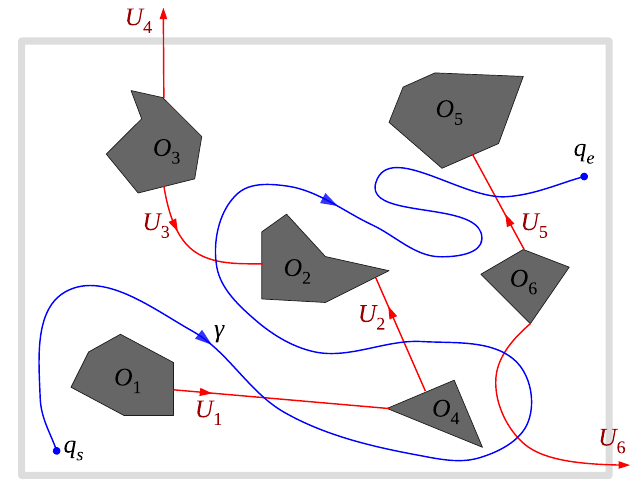
\includegraphics[scale=.4]{word_construction}
  \caption{The blue path yields the constructed word
    \(h(\gamma) = u_{1}^{-1} u_{6} u_{6}^{-1} u_{2} u_{3} u_{5}^{-1} =
    u_{1} u_{2} u_{3} u_{5}^{-1}\)
    \cite{bhattacharyaPathHomotopyInvariants2018}.}
  \label{fig:word-construction}
\end{figure}

Hershberger et. al. restrict
the search of \(\mathcal{C}\) to specific homotopy classes
\cite{hershbergerComputingMinimumLength1994}.

Yang et. al. \cite{yangEfficientSearchShortest2022} propose a method
to calculate the \(k\)-shortest non-homotopic paths by simplifiying
the topology and discarding \(2^{n} - k\) of the \(2^{n}\) possible
paths in a two dimensional environment with \(n\) obstacles.

Wu et. al. \cite{wuMultiRobotPathDeconfliction2020} propose a method
to deconflict paths of multiple robots in cluttered environments.
Sequencially each robot computes it's path. The order is determined by
the number of homology classes of paths of each robot.

A solution for a similar problem is shown by Wang
et. al. \cite{wangCoordinationfreeMultirobotPath2022}. They show a
solution to multi-robot path planning in complex cluttered
environments without inter-robot communication or coordination. The
approach assigns robots stochastically to different topological
classes and uses a potential field based controller to avoid local
obstacles.

\subsection*{Persistent Homology}
In \cite{bhattacharyaPersistentHomologyPath2015} the authors try to
solve the problem of how to threshold an occupancy grid map to get a
binary map for the use with classic path planning techniques. They use
persistent homology to get the homology class of paths that is
persistent over the widest range of threshold values.

\section*{Configuration Spaces with moving Obstacles}
In the thesis we want to apply the concept of persistent homology to
the problem of planning paths with moving obstacles using graph
search-based algorithms.


\bibliographystyle{plain} \bibliography{../bib/mybib}
\end{document}
